\section{Performance}

Performance evaluation of the automated subject classification component is
treated in section \ref{autoclasseval}.
Performance in terms of number of URLs treated per minute is of course
highly dependent on a number of circumstances like network load,
capacity of the machine, the selection of URLs to crawl, configuration
details, number of crawlers used, etc.
In general, within rather wide limits, you could expect the Combine
system to handle up to 200 URLs per
minute. Handle here means everything from scheduling of URLs, fetching
of pages over the network, parsing the page,
automated subject classification, recycling of new links, to storing the structured record in
a relational database. This holds for small simple crawls starting
from scratch to large complicated topic specific crawls with millions
of records.

\begin{figure}[htb]
\begin{center}
 \includegraphics[height=0.4\textheight]{CrawlerSpeed.ps}
\end{center}
\caption{Combine crawler performance.}
\label{crawlspeed}
\end{figure}

The prime way of increasing performance is to use more than one
crawler for a job. This is handled by the {\tt --harvesters } switch
used together with the {\tt combineCtrl start} command (for example\\
{\tt combineCtrl -jobname MyCrawl --harvesters 5 start}\\
will start 5 crawlers working together on the job 'MyCrawl'. The
effect of using more than one crawler on crawling speed is illustrated
in figure \ref{crawlspeed} below.

Configuration also have an effect on performance. In figure
\ref{config} performance improvements based on configuration changes are shown. The choice of
algorithm for automated classification turns out to have biggest
influence on performance, where \hyperref{algorithm 2}{algorithm 2 - section }{ -}{pos} ({\tt classifyPlugIn = Combine::PosCheck\_record} - Pos in figure \ref{config}) is much
faster than \hyperref{algorithm 1}{algorithm 1 - section }{ -}{std} ({\tt classifyPlugIn = Combine::Check\_record} - Std in figure \ref{config}). Tweaking of other configuration variables also have an effect
on performance but to a lesser degree. Tweaking consisted of not using
Tidy to clean HTML ({\tt useTidy = 0}) and not storing the original
page in the database ({\tt saveHTML = 0}).


\begin{figure}[htb]
\begin{center}
 \includegraphics[height=0.4\textheight]{Config.ps}
\end{center}
\caption{Effect of configuration changes on focused crawler performance.}
\label{config}
\end{figure}



